\documentclass[a4paper,10pt]{article}
\usepackage[fleqn]{amsmath}
\usepackage{amsfonts}
\usepackage{amssymb}
\usepackage{theoremref}
\usepackage[pdftex]{hyperref}
\usepackage{daa}
\usepackage{listings}
\usepackage{tikz}
\usetikzlibrary{arrows,decorations.pathmorphing,backgrounds,positioning,fit,petri}



\hypersetup{colorlinks,%
		citecolor=black,%
		filecolor=black,%
		linkcolor=black,%
		urlcolor=blue}

\title{
\begin{figure}[h]
\centering
\includegraphics[width=0.2\linewidth]{t}
\end{figure}
\textbf{Surubi}\\ Compilador para Tiger} %TODO: poner el pescado

\author{Carlos David Muñiz Chall\\Jesús Manuel Garnica Bonome}
\date{14 de abril 2017}

\begin{document}
	\maketitle

	\section{Descripción}
		
		Surubi es un compilador para el lenguaje de programación \textbf{Tiger} definido por \textit{Stephen A. Edwards}\cite{tlrm} con la modificaciones requeridas para el año 2017\cite{ol}. Este compilador está escrito en el lenguaje de programación \textit{C\#}, utilizando un reconocedor sintáctico generado por la herramienta \textit{Antlr 3.4}. A partir del fichero de entrada, el cual es el único argumento requerido, se genera un fichero que contiene código ensamblador listo para ser procesado por el ensamlador de \textit{NASM}.
		
	\section{Arquitectura}
		
		Durante la compilación interactuan tres componentes principales:
		\begin{itemize}
			\item Reconocedor sintáctico \\
				Este es el encargado de crear un Ábol de Sintaxis Abstracta(\textit{AST}) a partir del texto de entrada,
				la implementación por defecto fue hecha utilizando \textit{Antlr 3.4}
			\item Comprobador semántico \\
				Dedicado al chequeo statico de tipos y a la existencia en cada ámbito de los miembros utilizados,
				la implementación por defecto se llama \textit{DefaultSemanticChecker}.
			\item Emisor de código \\
				Provee una interfaz de instrucciones que permiten las acciones usuales en un lenguage de programación,
				la implementación por defecto \textit{NasmEmitter} produce código \textit{NASM}
		\end{itemize}
		
		La otra parte central en la arquitectura del compilador son los nodos del \textit{AST} cada uno cuenta con el siguiente conjunto de propiedades y métodos:
		\begin{itemize}
			\item line \\
			Linea donde fue reconocido el principio de la estructura que representa el nodo.
			\item column \\
			Posición en que comienza la estructura en la linea.
			\item Lex \\
			Para nodos atómicos, como los literales, es todo el texto asociado con la estructura que representan, en otro caso por lo general no se utiliza.
			\item CheckSemantics(Comprobador Semantico, Reporte de errores, Tipo esperado) \\
			Comprueba la correctitud semantica del nodo presente,
			el valor de retorno determina si el nodo actual pudo decidir el tipo de la etructura que represeta.
			\item GenerateCode(Emisor de Código, Reporte de errores) \\
			Utilizando las funciones provistas por el emisor genera código encargado de cumplir con la semantica del nodo.
		\end{itemize}
		
		Esta definición básica es extendida por dos definiciones más especializadas, expresiones y declaraciones.
		
		Expresiones, estas representan nodos que después de su ejecución devuelven un valor:
		\begin{itemize}
			\item Return \\
			Representa el tipo de retorno del valor, este es necesario para el chequeo estatico de tipos.
			\item ReturnValue \\
			Representa la información sobre donde %tilde?
			va a quedar el valor de retorno durante la ejecución.
			\item CanBreak \\
			Valor que indica si el nodo actual puede causar la salida temprana de un ciclo
		\end{itemize}
		
		Las declaraciones representan nodos que sólo añaden miembros al ámbito actual, para manejar las declaraciones cíclicas la comprobación semántica se extendió a dos faces, la fase adicional \textit{BindName} se encarga de añadir la información del miembro que representa, pudiendo estar incompleta, mientras que \textit{CheckSemantics} comprueba la coherencia de esta definición y la completa en caso de ser necesario.
		
		\subsection{Reconocedor Sintáctico}
		
		Al ser implementado con \textit{Antlr 3.4} este utiliza una gramática \textit{LL(*)}, por lo que las siguientes sintáxis presentan conflictos, donde la alternativa correcta no puede ser decidida por un autómata finito.
		
		\begin{itemize}
			\item [] lvalue:
			\begin{itemize}
				\item [] id
				\item [] lvalue . id
				\item [] lvalue [ expr ]
			\end{itemize} 
			\item [] lvalue := expr
			\item [] id (expr-list)
			\item [] id {field-list}
			\item [] id [ expr ] of expr
		\end{itemize}
		
		Aunque la herramienta utilizada provee facilidades como los predicados sintáticos para resolver este tipo de comflictos, la solución dada solo utiliza factorización izquierda.
		
		\begin{figure}[h]
			\centering
			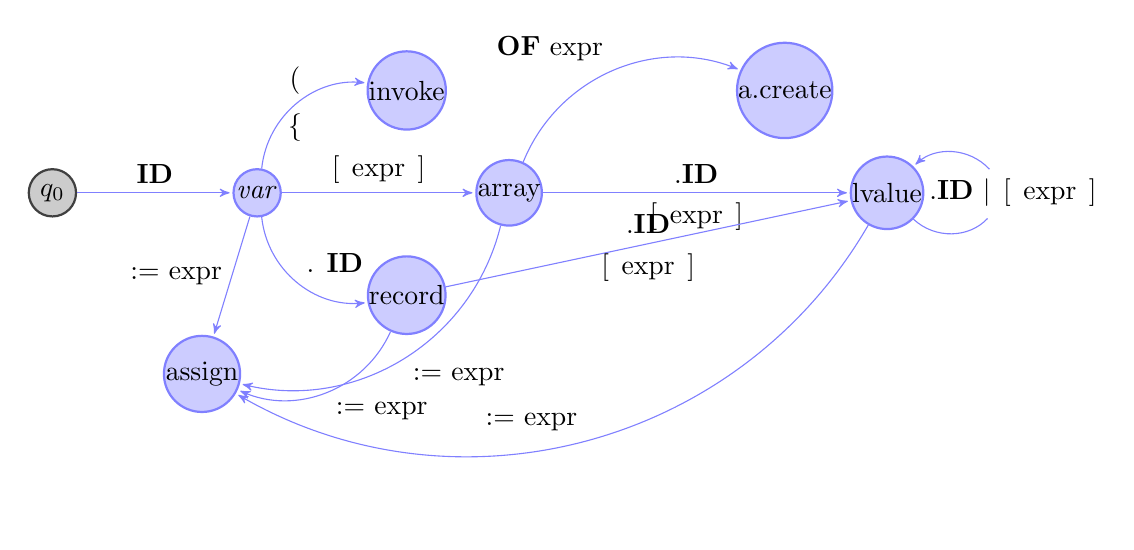
\begin{tikzpicture}
			[node distance=1.3cm,>=stealth',on grid,bend angle=45,auto,
			final/.style={circle,draw=blue!50,fill=blue!20,thick,inner sep=0pt,minimum size=6mm},		
			nonfinal/.style={final,draw=black!75,fill=black!20},
			every label/.style= {red}]
			
			\node [nonfinal](q0)                                 {$q_0$};
				\node (fq0r) [right=of q0, yshift=3mm]            {};
				\node (fq0rb) [below=of fq0r, xshift=3mm]         {};
				%\node (fo3) [below=of o1, xshift=-3mm]           {};
				
			\node [final](v)    [right=of fq0r, yshift=-3mm]  {\textit{var}}
				edge             [pre, draw=blue!50] node[swap] {\textbf{ID}} (q0);
				%edge             [pre, draw=blue!50, densely dashed] (o1);
			    \node (fvr) [right=of v, xshift=3mm]            {};
			    
				
			\node [final](i) [above=of fvr, xshift=3mm]      {invoke}
				edge             [pre,bend right, draw=blue!50] node[above,swap] {$\left(\right.$} node[below,swap] {$\left\lbrace\right.$}  (v);
				
			\node [final](a) [right=of fvr, xshift=3mm]      {array}
				edge             [pre, draw=blue!50] node[swap] {$\left[\right.$ expr $\left.\right]$}  (v);
				\node (far) [right=of a, xshift=3mm]            {};
				\node (farr) [right=of far, xshift=3mm]            {};
				
			\node [final](r) [below=of fvr, xshift=3mm]      {record}
				edge             [pre,bend left, draw=blue!50] node[swap] {. \textbf{ID}}  (v);
				
			\node [final](ass) [below=of fq0rb, xshift=3mm]      {assign}
				edge             [pre, draw=blue!50] node[left,swap] {:= expr}  (v)
				edge             [pre, bend right, draw=blue!50] node[swap] {:= expr}  (a)
				edge             [pre, bend right, draw=blue!50] node[swap] {:= expr}  (r);
				
			\node [final](l) [right=of farr, xshift=3mm]      {lvalue}
				edge             [pre, draw=blue!50] node[above, swap] {.\textbf{ID}} node[below,swap] {$\left[\right.$ expr $\left.\right]$}  (a)
				edge             [pre, draw=blue!50] node[above, swap] {.\textbf{ID}} node[below,swap] {$\left[\right.$ expr $\left.\right]$}  (r)
				edge             [post, bend left, draw=blue!50] node[swap] {:= expr}  (ass);
				
						
				\node (la) [right=of l, xshift=3mm]            {.\textbf{ID} $\left|\right.$ $\left[\right.$  expr $\left.\right]$}
					edge             [pre,-, bend left, draw=blue!50] (l)
					edge             [post, bend right, draw=blue!50] (l);
				
			\node [final](ac) [above=of farr, xshift=3mm]      {a.create}
				edge             [pre, bend right, draw=blue!50] node[swap] {\textbf{OF} expr}  (a);
			
			
				%edge             [post, draw=blue!50, densely dashed]   (o1);
			\end{tikzpicture}
			\caption{Automata para el reconocimiento de las producciones que comienzan por \textbf{ID}}
		\end{figure}		
		
		\pagebreak
		
		Producciones de la gramatica para lograr el automata anterior.
		\begin{itemize}
			\item lvalue-head:\\
				\textbf{ID} (invoke $\left|\right.$ \textbf{[}exp\textbf{]} array $\left|\right.$ . \textbf{ID} record $\left|\right.$ assign)?
			\item invoke:\\
				\textbf{(} argument-list? \textbf{)} $\left|\right.$ \textbf{$\lbrace$} field-list? \textbf{$\rbrace$}
			\item array:\\
				\textbf{OF} expr $\left|\right.$ lvalue
			\item record:\\
				lvalue
			\item lvalue:\\
				(\textbf{.ID} $\left|\right.$ \textbf{[}exp\textbf{]})* assign?
			\item assign:\\
				\textbf{:=} expr				
		\end{itemize}
		
		El resto de los conflictos fueron operadores binarios del tipo \textit{expr} \textbf{op} \textit{expr}, para los cuales se aplicó
		factorización izquierda reflejando la precedencia de forma explícita.
		
	\section{Comprobación Semántica}
		
		Durante la comprobación semantica cada nodo chequea a sus descendientes y luego comprueba que el tipo de retorno sea el adecuado.
		Para manejar el chequeo de los nodos que no devuelven ningún valor se introdujo el tipo \textit{void} y para la constante \textit{nil} el tipo \textit{null}, ninguno de los dos son explícitamente accesibles al código que se está compilando.
		
		Durante este proceso se trabaja con objetos que describen los miembros que serán generados en la siguiente fase.
		
		Miembro
		\begin{itemize}
			\item Name
			\item BCMMember\\
				Esta propiedad guarda el menegador generado por la declaración de este miembro, el cual es usado para referirse a el durante la generación de código.
			\item BCMBackup\\
				Indica si este miembro requiere de un \textit{BCMMember}, lo cual es el caso de todos los miembros excepto el tipo \textit{void} y el tipo \textit{null}.
		\end{itemize}
		
		Campo, es la abstración que representa una zona de memoria, vaiables y constantes, extiende miembro.
		\begin{itemize}
			\item Type\\
				Información sobre el tipo del campo.
			\item Cosnt\\			
				Indica si este miembro es de solo lectura.
		\end{itemize}
		
		Funciones, extiende miembro.
		\begin{itemize}
			\item Parameters\\
				Lista con el tipo y nombre de los parámetros que recive la función, el orden de la lista coincide con el orden de la declaración y de las invocaciones.
			\item Return\\			
				Tipo del valor de retorno, si es un procedimiento el tipo es \textit{void}.
		\end{itemize}
	
		Tipos, extiende miembro.
		\begin{itemize}
			\item Members\\
				Lista con el tipo y nombre de los campos del registro que representa el tipo.
			\item ArrayOf\\
				Tipo de los elementos del array que representa el tipo, etsta propiedad y \textit{Members} no deben ser difrenetes de \textit{null} las dos en el mismo tipo.
			\item Complete\\
				Indica si la descripción del tipo ha terminado, solo puede ser falsa en fases intermedias de la comprobacion de declaraciones.
			\item TypeId\\			
			Identificador único para cada tipo, máximo $2^{128}$ tipos.
		\end{itemize}
				
		\subsection{Expresiones}
		Al terminar la comprobación semántica de un nodo expresión se deben cumplir las siguientes condiciones:
		\begin{itemize}
			\item Si el valor de retorno fue verdadero entonces las propiedades \textit{Return} y \textit{ReturnValue} deben estar correctmente asignadas, \textit{Return} nunca debe ser nula.
			\item Si y solo si \textit{Return} es el tipo \textit{void} entonces \textit{ReturnValue} es nula.
			\item Si \textit{CanBreak} es verdadera \textit{Return} es el tipo \textit{void}.
			\item El valor de retorno es falso si y solo si no se puede determinar el valor de \textit{Return}.
		\end{itemize}
		
		Como consecuencia de esto existen nodos que nunca devuelven falso en su chequeo semántico, como lo son los operadores de enteros los que siempre devuelven \textit{int}, por esta razón el chequeo semántico se considera fallido si se agregan errores al reporte.
		
		\subsection{Declaraciones}
		
		El chequeo semántico de las declaraciones se dividió en dos fases para manejar las secuencias de declaraciones del mismo tipo.
		La fase de \textit{BindName} es la primera que se ejecuta excepto en el caso de la declaración de los parámetros de una función.
		Como las dos fases tienen significados ligeramente diferentes según el tipo de declaración serán expuestas por separado.
		
		En las declaraciones de variables \textit{BindName} no tiene efecto alguno, mientras que \textit{CheckSemantics} hace las comprobaciones y añade el descriptor al ámbito actual. Para los parámetros \textit{CheckSemantics} hace la comprobación estática de tipos y \textit{BindName} añade el descriptor al ámbito actual.
		
		Las funciones se comportan igual que los parámetros pero en orden inverso, para lograr el efecto de las secuencias de declaraciones.
		
		Los tipos usan \textit{BindName} para añadir el descriptor al ámbito actual, solo que si los tipos de los que depende esta declaración no existen el descriptor no es añadido, excepto para los registros los cuales lo añaden marcándolo como incompleto. \textit{CheckSemantics} completa los descriptores y hace los chequeos de tipo, para lo que necesita ser ejecutado después que el chequeo semántico de las declaraciones de la que depende. El orde de ejecución de \textit{CheckSemantics} y de la generación de código en las declaraciones se determina mediante un orden topológico de sus dependencias, comenzando por las que tienen $1$ dependencia. Las declaraciones sin dependencias son comprobadas al final.
		
		\section{Generación de Código}
		
		Para la generación de código se diseño una abstracción del comportamiento de un equipo de cómputo, el conjunto de instrucciones que deben ser implementadas se puede resumir en el siguiente:
		
		\begin{itemize}
			\item Instrucciones aritméticas.
			\item Añadir Constantes
			\item Creación de variables.
			\item Creación de objetos, registros y vectores.
			\item Creación de tipos.
			\item Enlaze con objetos, funciones y tipos de una biblioteca estandar.
			\item Etiquetas y saltos absolutos y condicionales
			\item Ámbitos locales y de función
			\item Emisión de errores
			\item Invocación de funciones
			\item Valores de retorno de funciones y parámetros			
		\end{itemize}
		
		La implementación se hizo generando ensamblador, la biblioteca estandar está mayormente implentada en ensamblador también con algunas funciones en \textit{C}, para esto fue necesario manejar durante toda la generación dos protocolos de invocación:
		
		\begin{itemize}
			\item cdcall\\ %check
				Los parámetros se pasan en la pila de derecha a izquierda y el valor de retorno se deja en \textit{EAX}, el que invoca es el que libera la pila después de la invocación. También utilizado para enlazar con las funciones de la estandar de \textit{C}.
			\item tiger-call\\
				Es una extensión de \textit{cdcall} para manejar las clausuras de las funciones de tiger.
				Cada ámbito de tiger tiene como pimer valor en la pila un puntero al ámbito que lo contiene, para poder utilizar los miembros que declaran sus antecesores. Las funciones de tiger tambien cumplen esto, pero el puntero debe ser almacenado junto con la posición de la función después de su declaración para se pasado como parámetro extremo derecho en cada invocación. Dentro de la función se guarda el puntero del ámbito que la invocó, para ser reestablecido al finalizar esta, y el último parámetro pasa a ser el puntero al ámbito contenedor.
		\end{itemize}
		
		La solución a los saltos hacia posiciones desconocidas es un sistema de reservación de etriquetas que no utiliza \textit{backpatch}, cada nodo que le interece permitir saltos a una etiqueta puesta por él, debe hacerla publica para sus descendientes durante la comprobacián semántica, en el caso de los ciclos se utiliza \textit{LoopScopeDescriptor} para que cualquier nodo implementando una salida temprana pueda conocer la etiqueta final de ciclo.
		
		Para obtener un ejecutable a partir de la salida es necesario proveer un ensamblador de \textit{NASM} y un enlazador, junto con el proyecto se provee una carpeta con el ensamblador y el enlazador para \textit{Windows}, el comportamiento por defecto puede ser modificado mediante argumentos en el comando de entrada.
		
	\bibliography{sources}
	
\end{document}